\documentclass[11pt,a4paper]{article}
\usepackage[T1]{fontenc}
\usepackage[utf8]{inputenc}
\usepackage{lmodern}
\usepackage[a4paper,margin=22mm,headheight=15pt]{geometry}
\usepackage{amsmath,amssymb,booktabs,array,tabularx,graphicx,xcolor,tikz}
\usetikzlibrary{arrows.meta,positioning}
\usepackage[numbers,sort&compress]{natbib}
\usepackage[unicode,colorlinks=true,linkcolor=black,citecolor=black,urlcolor=blue]{hyperref}
\definecolor{ink}{HTML}{153348}
\definecolor{accent}{HTML}{CE164E}
\definecolor{muted}{HTML}{546671}
\setlength{\parindent}{0pt}
\setlength{\parskip}{6pt}
\setlength{\emergencystretch}{4em}
\renewcommand{\arraystretch}{1.17}
\newcommand{\pagehead}[2]{\clearpage{\small\color{accent}\textbf{#1}}\par\vspace{3mm}{\LARGE\color{ink}\textbf{#2}}\par\vspace{3mm}}
\newcommand{\sub}[1]{\par\vspace{2mm}{\large\color{ink}\textbf{#1}}\par}
\newcommand{\evidence}[1]{\par\vspace{2pt}{\raggedright\footnotesize\color{muted}Projektbeleg: #1\par}}
\newcolumntype{Y}{>{\raggedright\arraybackslash}X}
\hypersetup{pdftitle={KUKA KR16 L6: Physik und Daten als Healthy-Referenz},pdfauthor={Mounir Belboualia}}

\hypersetup{pdftitle={KUKA KR16 L6: Wissenschaftlicher Fortschrittsbericht, 31.10.2026}}
\newcommand{\src}[1]{{\footnotesize\color{muted}[#1]}}
\begin{document}
{\small\color{accent}\textbf{FORSCHUNGSSTAND 31.10.2026}}\par
{\LARGE\color{ink}\textbf{KUKA KR16 L6:\\Physik und Daten als Healthy-Referenz}}\par
Mounir Belboualia\par
\sub{1. Forschungsfrage und Ausgangspunkt}
Kann ein physikalisch-datengetriebener Ansatz die Sensorsignale eines Industrieroboters besser erklären und langfristig zur zuverlässigen Erkennung von Zustandsveränderungen beitragen?

Der bisherige Befund ist differenziert: Ein mechanisches Modell verbessert einen eng gefilterten Healthy-Vergleich geringfügig. Auf nativen Beschleunigungen ist der zusätzliche Nutzen gegenüber einem rein datengetriebenen Modell sehr klein. Die bisherigen Alarmschwellen übertragen sich nicht zuverlässig. Diese Ergebnisse begründen gezielte Prüfungen der Messabbildung und der zeitlichen Generalisierung, keine bereits einsatzfähige Verschleißdiagnose.

\sub{Sheffield-AWT und Ereignisphasen}
James Moore und Daniela Sawyer berichten den Accelerated Wear Test (AWT) eines KUKA KR16 L6 am AMRC. J3 wurde über 13 Monate isoliert mit 100\,\% vorgegebener Geschwindigkeit/Beschleunigung sowie maximaler Nutz- und Zusatzlast hin- und herbewegt. Wiederkehrende Fingerprints umfassen J3 und das Kontrollgelenk J2 bei 10/50/100\,\%. Erfasst wurden Beschleunigung, Phasenstrom und Temperatur. \src{S1--S3}

\begin{tabularx}{\linewidth}{p{3.0cm}Y}
\toprule Grenze laut README & Ab hier vorgeschlagene Phase\\\midrule
19.01.2023, 19:13 & Oil Leaking\\
20.04.2023, 16:32 & Oil Partially Drained\\
24.04.2023, 13:00 & Oil Fully Drained\\
26.04.2023, 13:15 & Crashed\\\bottomrule
\end{tabularx}
Die Quellenzeitangaben erhalten hier keine nachträglich angenommene Zeitzone. Es handelt sich um dokumentierte Phasengrenzen, nicht um unabhängig erkannte Schadenszeitpunkte. Nach zunächst unauffälligen zwölf Wochen führten die Autoren Abkühlungen ein. Das README empfiehlt wegen Aufwärmeinflüssen eine J3-Mitteltemperatur von mindestens 39,5\,$^\circ$C für vergleichbare Fingerprints. Eine spätere Geräuschänderung wird hier mangels neu geprüften Volltextbelegs nicht behauptet. \src{S3}

\sub{2. Die Datenarchitektur ermöglicht kontrollierte Versuche}
ORDA-/Figshare-Metadaten und ein ZIP-Range-Leser erschließen einzelne MAT-Dateien, ohne Monatsarchive vollständig zu laden. Der Loader trennt bewegtes Gelenk, Geschwindigkeit und Sensor. Jeder Bewegungsblock enthält beide dreiachsigen Beschleunigungssensoren. Struktur-, Zeit- und Integritätsprüfungen gehen Modellvergleichen voraus. \src{P1}

\textbf{Datenbasis:} 4.659 MAT-Einträge im Manifest, 383,52 GB für alle dort aufgeführten entfernten Dateien; davon rund 383,43 GB ZIP-Archive. Lokal liegen 47 Healthy-MATs vor. Das ist ein kleiner, ausschließlich als Healthy vorgeschlagener Ausschnitt. Abtastraten: anfangs 10.240, später 25.600 Hz für Beschleunigung; nominal 1.000 Hz Strom und 1 Hz Temperatur. Messdatei-Properties bleiben maßgeblich. \src{S2,S3,P1}

\pagehead{MODELLIERUNG UND ERSTE PRÜFUNG}{3. Newton-Grey-Box und korrigierte Studie V2}
\sub{Fragestellung und Modellannahmen}
Lässt sich die gemessene Beschleunigung aus der Gelenkmechanik erklären? Unter isolierter J3-Bewegung, festem J2 und Starrkörperannahmen wurde der Drehimpulssatz als effektive Bewegungsgleichung formuliert:
\[
\ddot\theta_3=\kappa_0+\kappa_1u(t)-\gamma\dot\theta_3
-\lambda_c\cos\theta_3+\lambda_s\sin\theta_3.
\]
Sieben globale Größen sind $\kappa_0,\kappa_1,\gamma,\lambda_c,\lambda_s,\rho_x,\rho_y$. Die letzten beiden beschreiben den effektiven Sensorhebelarm. Hinzu kommen $\theta_3(0)$ und $\dot\theta_3(0)$. Numerische Integration liefert Winkel, Winkelgeschwindigkeit und Winkelbeschleunigung; die Starrkörperkinematik liefert daraus die Sensorvorhersage. Für einen Punkt mit Hebelarm $r$ gilt unter diesen Annahmen
\[
a_S=a_O+\alpha\times r+\omega\times(\omega\times r).
\]
Die unbekannte Rotation $Q$ und die Messkette verbinden Körper- und Sensorkoordinaten. Im historischen Code gilt für Zeilenvektoren $f_{\mathrm{sensor}}=f_{\mathrm{body}}Q$. Der Strom $u(t)$ ist ein empirischer Antriebsproxy, kein gemessenes Drehmoment. Die spezifische Kraft ist von der kinematischen Beschleunigung und einer idealen statischen Gravitationsmessung zu unterscheiden. \src{P2}

\sub{Schätzung und erster negativer Befund}
Least Squares mit numerischen Suchgrenzen minimierte die quadrierten Residuen. Der Pilot verwendete einen Trainingsfingerprint vom 25.10. und eine spätere Aufnahme vom 01.11.2022. Über 24 diskrete Rotationskandidaten wurden je zwei Starts gerechnet. Ein günstiger Fit beweist weder ein globales Minimum noch physikalisch richtige Parameter.

\begin{tabularx}{\linewidth}{Y r r}
\toprule Auswertung & Modell-RMSE & Null-RMSE\\\midrule
Pilot, eine spätere Aufnahme & 0,014982 & 0,014707\\
V2, zehn QC-geeignete Testtage & 0,013822 & 0,014268\\\bottomrule
\end{tabularx}
\smallskip Alle Werte in m/s$^2$. Beide Zeilen betreffen gefilterte Offline-Ziele; Datenbasis, Randfenster und Verarbeitung unterscheiden sich. Im Pilot war das Modell rund 1,87\,\% schlechter als Null. V2 verbesserte die Nullreferenz um 3,13\,\%. Ein direkter kausaler Vorher-nachher-Effekt einzelner Korrekturen ist damit nicht isoliert. \src{P2,P3}

\sub{Warum war die Korrektur notwendig?}
Der Audit deckte unter anderem asymmetrische Filterung auf. V2 verwendete konsistente Mess-/Modelloperatoren im Analyseband 0,7--5 Hz, sechs Trainingstage, drei Validierungstage und zwölf spätere Testkandidaten. Zwei erfüllten die Temperatur-QC nicht; zehn gingen in den Score ein. Freeze vor Testzugriff, gemeinsame Trainings-Anfangszustände und Tagesauslassungen begrenzten Anpassung und prüften Stabilität. Das bedingte 95\,\%-Blockintervall des mittleren RMSE lautet [0,012982; 0,014626] m/s$^2$. Seine Gültigkeit hängt von den Abhängigkeitsannahmen ab. Gegenüber der Zeitvorlage blieb der Vorteil uneindeutig. \src{P3}

\textbf{Identifizierbarkeit:} Zwei verschiedene rechtshändige $Q$ erzeugen bei passend transformierten Parametern dieselbe Vorhersage. Dieses konkrete Gegenbeispiel widerlegt globale Eindeutigkeit. Es beweist keine allgemeine lineare Familie aller Parameter. Eine externe Winkel-/Montagereferenz bleibt nötig. \src{P2}

\pagehead{ANTRIEB UND UNABHÄNGIGE BEWEGUNGSREFERENZ}{4. Stromproxies und Videoanalyse}
\sub{Kann eine andere Strombeschreibung die Vorhersage verbessern?}
Die RMS-bezogene Strommesskette erhält weder den vorzeichenbehafteten $i_q$-Strom noch das reale Gelenkmoment. Deshalb wurden effektive Eingänge verglichen: H0 konstant, H1 direkt, H3 verzögert, H6B geglättet und H6C verzögert plus geglättet. Der Mechanik-/Beobachtungsansatz blieb dabei kontrolliert fest; Eingangskoeffizienten und Dynamik wurden angepasst. \src{P4}

\begin{tabularx}{\linewidth}{l Y r}
\toprule Modell & Eingang $z(t)$ & Interner RMSE\\\midrule
H0 & Konstanter effektiver Eingang & 0,015215\\
H1 & $z=u$ & 0,014760\\
H3 & $z=u(t-\Delta)$ & 0,013839\\
H6B & $T\dot z+z=u$ & 0,014236\\
H6C & $T\dot z+z=u(t-\Delta)$ & 0,013839\\
Zeitvorlage & Beschleunigung aus übrigen Trainingstagen & 0,013703\\\bottomrule
\end{tabularx}
\smallskip Mittel der Tages-RMSE in m/s$^2$, J3/50\,\%, sechs bereits bekannte Entwicklungstage, Leave-One-Day-Out. H0 ist kein Nullsignal. Die Vorlage verwendet jeweils die übrigen fünf Tage. Die Prüfung ist intern, weil Pipeline und Ausgangsmodell auf diesen Tagen entwickelt wurden. \src{P4}

H3 senkte den internen Fehler gegenüber H1 um etwa 6,24\,\%. Die später nativ geprüfte Verzögerung lag bei rund 72 ms. Daraus folgt keine identifizierte Motor- oder Messkettenverzögerung: Filter, Synchronisation und Modellfehler können denselben Effekt erzeugen. Die direkte Beschleunigungsvorlage blieb etwas besser. Eine stabile Übertragung auf andere Geschwindigkeiten wurde nicht nachgewiesen. H6C brachte keinen klaren Zusatznutzen gegenüber H3. \src{P4}

\textbf{Phase 4R blieb beim Vorabcheck stehen.} Fünf zusätzliche Healthy-Kandidaten waren nicht lokal vorhanden. Es erfolgte keine neue unabhängige numerische Validierung. Die vorhandenen nativen Diagnosen auf den sechs Entwicklungstagen sind davon getrennt. \src{P5}

\sub{Kann das Video die latente Gelenkbewegung unabhängig prüfen?}
Das mechanische Modell rechnet zuerst $\theta$, $\dot\theta$ und $\ddot\theta$, wurde aber primär an Beschleunigungen bewertet. Eine unabhängige Winkelreferenz sollte diese Zwischenstufe prüfen. Aus dem ORDA-Video wurden 2.341 Bilder bei 30 Bildern/s ausgewertet. Verfolgung, Farberkennung und Bildgeometrie untersuchten Bewegungsabschnitte und mögliche Umkehrpunkte. \src{P6}

\textbf{Ergebnis und Grenze:} J2-/J3-Abschnitte konnten qualitativ eingegrenzt werden. Unsichere Kamerakalibrierung und Gelenkpunkte sowie Trackingfehler verhinderten belastbare physikalische Winkel und deren Ableitungen. Die Videozeit ist nicht nachweislich mit einer bestimmten MAT-Datei synchronisiert. 2.341 Bilder sind ein Film, nicht 2.341 unabhängige Experimente.

\textbf{Folgerung:} Weder Stromproxy-Optimierung noch Bildverfolgung lösten die fehlende unabhängige Zustandsreferenz. Deshalb wurden anschließend die direkt beobachtbare Signalgeometrie und die mechanischen Modellannahmen getrennt untersucht.

\pagehead{SIGNALGEOMETRIE UND MECHANIK}{5. PCA, Montage und gekoppelte Dynamik}
\sub{Welche räumliche Information steckt tatsächlich im Signal?}
Phase C wertete 26 Fingerprints vom 01. und 03.11.2022 aus: sechs Bewegungsbedingungen und zwei dreiachsige Sensoren, insgesamt 312 Fälle. Mittelwertbereinigte Kovarianz/PCA, volle Spektren und zusätzliche Frequenzbänder trennten Rohsignalstruktur und niederfrequente Geometrie. Die spätere Phase C.2 konzentrierte sich auf 104 Fälle bei 10\,\% Geschwindigkeit. \src{P7}

Für eine positive semidefinite Kovarianz mit $\lambda_1\geq\lambda_2\geq\lambda_3$ gilt exakt:
\[
\lambda_3=0\ \land\ \lambda_2>0\quad\Longleftrightarrow\quad\operatorname{rang}(\Sigma)=2.
\]
Dann ist die Normalenachse bis auf das Vorzeichen eindeutig. Bei verrauschten Daten müssen zweite Anregung, Eigenwertabstand und Richtungsstabilität gemeinsam betrachtet werden. Richtungsvergleiche verwenden $\arccos(|n_1^\top n_2|)$. Der ideale Rangbeweis ist kein Nachweis einer realen mechanischen Sensorausrichtung.

\begin{tabularx}{\linewidth}{Y r}
\toprule C.2: Sensor J2 bei J2/10\,\% & Beobachtung\\\midrule
LP5, 1 s Randbeschnitt: median $\lambda_2/\lambda_1$ & 0,418\\
Median $\lambda_3/\lambda_2$ & 0,00180\\
Normalenwinkel zwischen den zwei Tagen, Median & 1,11$^\circ$\\
95\,\%-Quantil dieser Winkel, kein Konfidenzlimit & 3,15$^\circ$\\\bottomrule
\end{tabularx}
\smallskip LP5 bedeutet hier Vorwärts-/Rückwärts-Tiefpass bei 5 Hz ohne Hochpass, nach Antialias-Resampling; es ist nicht das Band 0,7--5 Hz. Der Ebenenkandidat ist in lokalen Sensorkoordinaten reproduzierbar, hängt aber von Zeitabschnitt und Frequenzwahl ab. Im engeren Band wird derselbe Fall stark einachsig. Die vielen Fingerprints liefern nur zwei Versuchstage. \src{P7}

Das unabhängige Montageaudit bestätigte keine quantitative Rotation in das mechanische Bezugssystem. Eine PCA-Normale darf diese fehlende Kalibrierung nicht ersetzen. Peaks um 8 kHz sind empirische Spektralbefunde; ihre Ursache und die Übertragung der Messkette sind nicht als Getrieberesonanz identifiziert. \src{P7,P8}

\sub{Welche Mechanik fehlte im einfachen J3-Modell?}
Die Erweiterung formuliert J2 und J3 mit den vereinbarten absoluten Winkeln. Euler--Lagrange und eine unabhängige Newton--Euler-Bilanz berücksichtigen Schwerpunktversatz $y_2$, Reibungsmatrix und Momententransformation. Die Beziehung $C=LV/g_0$ reduziert eine kollineare Parameterbasis. Symbolische Identitäten und synthetische Rechenprüfungen bestätigen die Konsistenz unter den Modellannahmen. \src{P9}

Für die bevorzugte J2-Arbeitshypothese $H_A$ bleibt $\theta_3$ absolut konstant; für J3 wird $\theta_2=\pi/2$ angenommen. Diese Vorgaben sind keine metrisch kalibrierte Videomessung. PCA allein entscheidet weder $H_A$ noch die konkurrierende Hypothese $H_B$. Frühere rotationsinvariante Norm-/Profilversuche überwanden die Identifikationsgrenzen ebenfalls nicht. \src{P9,P10}

\textbf{Folgerung:} Konsistente Gleichungen sind eine notwendige Modellvoraussetzung, aber nicht hinreichend für identifizierte Roboterparameter. Die weitere Forschung musste prädiktiven Nutzen und mechanische Interpretation getrennt prüfen.

\pagehead{STATISTISCHE UND FREQUENZBEZOGENE ERWEITERUNG}{6. V3 und V4 prüfen komplementäre Ziele}
\sub{V3: Wann liefert Strom zusätzliche Vorhersageinformation?}
V3 kombinierte die vorhandene Mechanik mit Maximum-Likelihood-Schätzung (MLE), regularisierenden MAP-Priors und expliziten Fehlerannahmen. Sechs Trainingstage und drei bekannte spätere Validierungstage wurden chronologisch getrennt. AR-Fehlerstrukturen berücksichtigten zeitliche Abhängigkeit, beseitigten sie aber nicht vollständig. MAP liefert hier einen Punktmodus unter gesetzten Priors, keine automatisch gültigen Unsicherheitsintervalle. \src{P11}

Im gefilterten Offline-Vergleich schlug keines der neuen mechanisch strukturierten Modelle V2. Ein separater Kausalzweig prüfte 100-ms-Vorhersagen anhand vergangener Beschleunigung, mit und ohne Strom. Auf den drei bekannten Tagen sank der mittlere Fehler durch Strom für J3 um 4,004\,\% und für J2 um 27,588\,\%. Das ist ein explorativer prädiktiver Mehrwert im jeweiligen Regime, keine kalibrierte Momentenübertragung. \src{P11}

\textbf{Wesentliche Einschränkung:} Der Zielfilter hat bei 1--4 Hz eine Gruppenlaufzeit von ungefähr 0,26--0,54 s. Ein Horizont von 100 ms für das gefilterte Signal bedeutet deshalb keinen 100-ms-Warnvorlauf gegenüber der ungefilterten Bewegung. Die Synchronisation unterschiedlicher Messgeräte bleibt unkalibriert.

\sub{V4: Welche native Schwingungsstruktur ist reproduzierbar?}
V4 untersuchte alle 47 lokalen Dateien, 282 Bewegungsblöcke und 1.692 Achsenaufnahmen mit Welch-Leistungsdichten, zeitabhängigen Bandenergien und Healthy-Referenzen. Es gab keine pauschale 5-Hz-Beschränkung. Sechs Trainingstage, drei Kalibriertage und zwölf bekannte spätere Tage bildeten den Vergleich; die zusätzlichen 26 explorierten Dateien wurden nicht als weitere Trainingstage gezählt. \src{P12}

\begin{center}
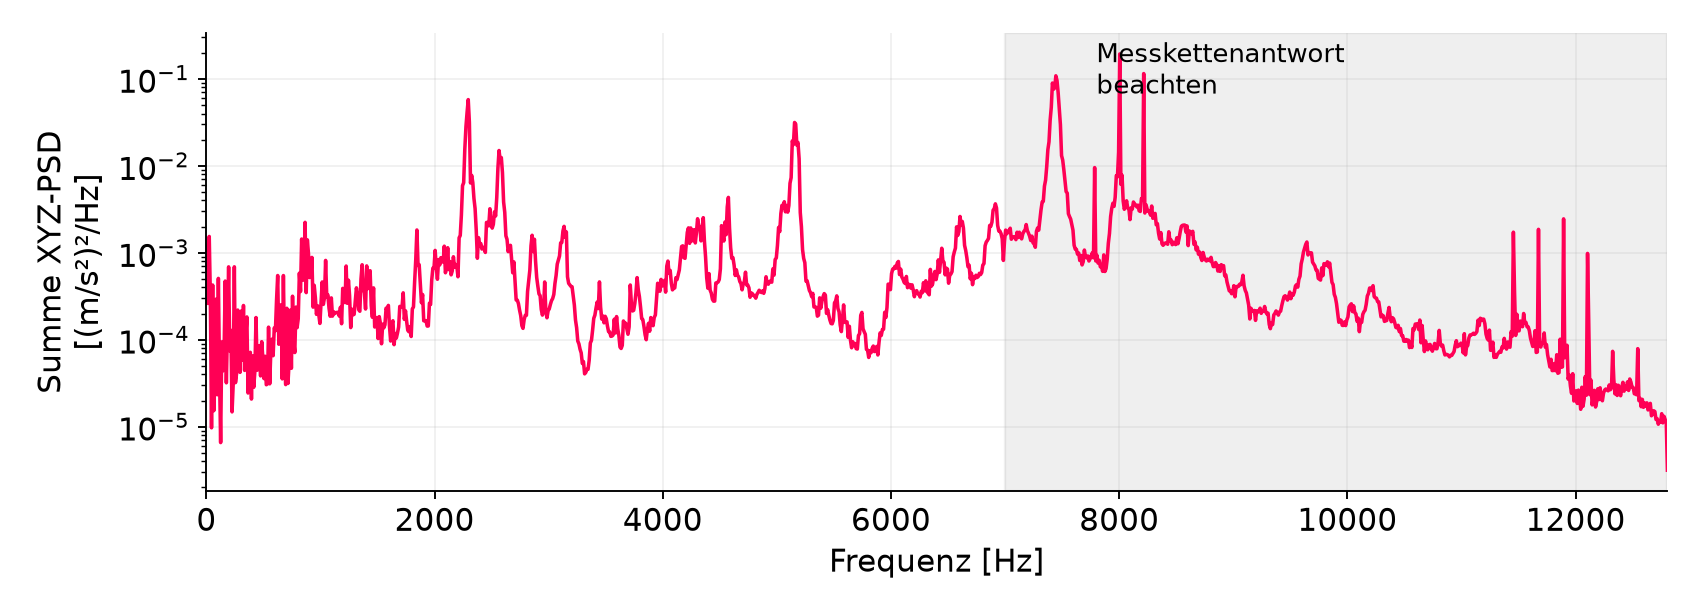
\includegraphics[width=0.86\linewidth,height=4.1cm,keepaspectratio]{spectrum.png}
\end{center}
{\footnotesize Gespeicherte PSD-Ableitung, Fingerprint 01.11.2022 14:31:59, J3/50\,\%, Sensor J3. Darstellung bis Nyquist; hohe Frequenzen sind nicht pauschal physikalisch kalibriert. Keine erneute Spektralberechnung.}

Die Prognose zukünftiger 0,5-s-Bandenergie im Bereich 20--4.000 Hz verringerte die Log-RMSE je nach Bewegungsbedingung um 0,34--9,18\,\% gegenüber der Zeitvorlage. Strom brachte keinen durchgängigen Zusatznutzen. Diese Fehler sind weder Beschleunigungs-RMSE noch eine unmittelbar vergleichbare Verbesserung von V2. Die V4-Alarmschwelle wurde auf 3/12 späteren Healthy-Aufnahmen überschritten. \src{P12}

\textbf{Folgerung:} Niederfrequente Dynamik, native Wellenform und Bandenergie beantworten unterschiedliche Fragen. Der nächste kontrollierte Vergleich musste Physik und Datenmodell auf demselben nativen Ziel prüfen.

\pagehead{GLEICHES NATIVES ZIEL FÜR ALLE MODELLE}{7. V5: kleiner Physikmehrwert, unzuverlässige Alarme}
V5 vergleicht vier Modelle auf J3/50\,\%, Sensor J3 XYZ. Sechs Trainingstage und drei Kalibriertage gehen zwölf historisch bekannten späteren Healthy-Tagen voraus. Modelle und Schwellen wurden vor dieser Evaluation eingefroren. Bekannte Daten werden dadurch nicht zu einem neuen Blindtest. \src{P13}

\begin{tabularx}{\linewidth}{l Y r}
\toprule Modell & Vorhersageprinzip & RMSE [m/s$^2$]\\\midrule
Null & Nullsignal & 2,832966\\
Vorlage & Healthy-Zeitvorlage & 3,009817\\
A & Direktes autoregressives Modell & 1,452605\\
B & Deterministische mechanische Sensorbaseline & 2,833019\\
C & B plus autoregressives Residualmodell & 1,452393\\
D & B plus stochastischer Winkelzustand/Kalman & 2,821173\\\bottomrule
\end{tabularx}
\smallskip Mittel der Tages-RMSE im gemeinsamen nativen Fenster 1,5--7 s; Ein-Schritt-Horizont 39,06 $\mu$s. A/C verwenden gewählte AR-Ordnung 24. Die Tabelle zeigt MLE-Varianten; untersuchte MAP-Priors ändern die Rangfolge nicht. D nutzt eine Kalman-Likelihood für einen latenten Winkelprozess. \src{P13}

C ist gegenüber A um 0,0146\,\% besser. Das ist ein numerischer Befund, kein überzeugender praktischer Nachweis mechanischen Zusatznutzens. Bei 10/100/500 ms freien Vorhersagen fehlt ein praktisch relevanter Abstand zur Nullvorhersage. D erreicht die gesetzte 4-kHz-Parametergrenze; das identifiziert keine reale Eigenfrequenz. Die native RMSE liegt auf einer anderen Zielskala als die 0,7--5-Hz-RMSE von V1/V2.

\begin{center}
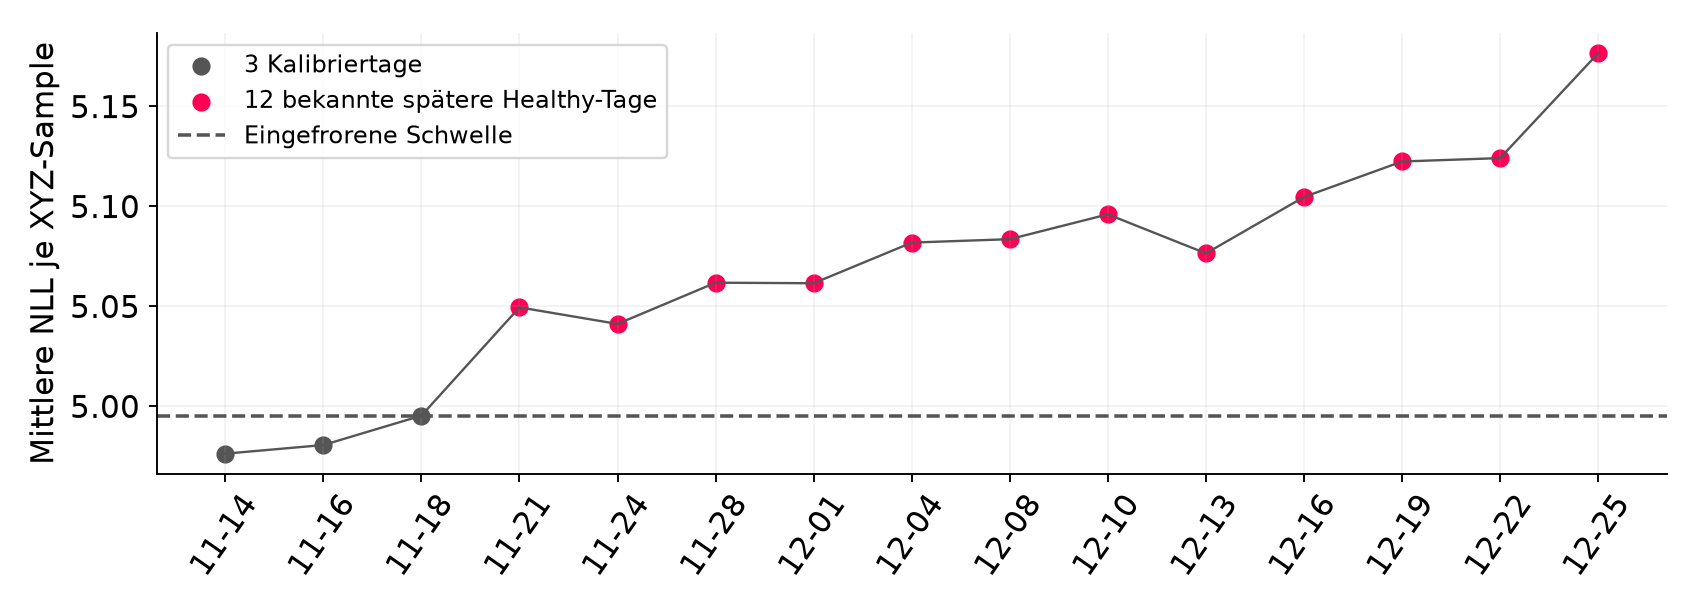
\includegraphics[width=0.88\linewidth,height=4.2cm,keepaspectratio]{alarm.png}
\end{center}
{\footnotesize Bestehende V5-Auswertung für Modell A: drei Kalibriertage und zwölf bekannte spätere Healthy-Tage. Die Maximalschwelle wurde nicht nachträglich korrigiert.}

\textbf{Alle zwölf späteren Healthy-Aufnahmen lösen bei A, B, C und D Alarm aus.} Bezogen auf die vorgeschlagenen Healthy-Labels sind dies Fehlalarme. Der negative Log-Likelihood-Score (NLL) beschreibt die Unvereinbarkeit mit dem angenommenen Fehler-/Referenzmodell, nicht automatisch Verschleiß. Temperatur, Messkette und zeitlicher Verteilungswandel sind mögliche, nicht identifizierte Ursachen. Die V4-Quote von 3/12 nutzt andere Scores und ist kein kontrollierter direkter Verfahrensvergleich.

\textbf{Folgerung:} Niedrige Kurzfristfehler reichen nicht zur zuverlässigen Alarmkalibrierung. Eine Freigabe von Verschleißerkennung, Restlebensdauer oder Wartungsentscheidungen folgt aus V5 nicht.

\pagehead{ERKENNTNISSE UND GEPLANTE FORTSETZUNG}{8. Langzeitprüfung und Forschungsbedarf}
\sub{Was ist erreicht, was bleibt offen?}
\begin{tabularx}{\linewidth}{Y Y}
\toprule Erreicht im jeweiligen Geltungsbereich & Noch nicht nachgewiesen\\\midrule
Reproduzierbarer selektiver Datenzugriff und Schema-/Zeitprüfungen & Vollständig extern bestätigte Uhren-/Messkettenübertragung\\
Newton-Modell, Integration und empirische Schätzungen & Eindeutige reale Winkel, Montage und physikalische Parameter\\
Systematische Baseline- und Modellvergleiche & Robuste Übertragung über Geschwindigkeit und Temperatur\\
PCA-/Spektralbefunde und statistische Healthy-Referenzen & Trennung von Alterung, Betrieb und Sensoränderungen\\
Symbolische und numerische Mechanikprüfungen & Physikalische Kalibrierung oder allgemeiner Roboternachweis\\
Dokumentierte negative Alarmprüfung & Kontrollierte Fehlalarmrate, Wartungszeitpunkt oder RUL\\\bottomrule
\end{tabularx}

\sub{Nächster empirischer Schritt: vollständiger Langzeitverlauf}
\textbf{Geplant, hier nicht ausgeführt:} Weitere Aufnahmeblöcke über Healthy-, Ölverlust-, Ölentleerungs- und Crash-Phasen erschließen. Ein eingefrorenes Protokoll definiert Zielgröße, Betriebsbedingungen, Qualitätsregeln und Ereignisfenster vor dem Scoring. Keine nachträgliche Auswahl günstiger Aufnahmen und kein pauschaler Komplettdownload.

Zuerst folgt eine breitere Healthy-Kalibrierung mit reservierten Prüfblöcken, danach der einmalige Ereignisvergleich bei vergleichbaren Geschwindigkeiten und Temperaturen. Aufnahme-/Tagesblöcke berücksichtigen zeitliche Abhängigkeit. Abkühlungen, Datenlücken, Messratenwechsel und die J2-Kanaländerung um 4.200 h gehören in die Prüfung. Phasenlabels sind keine präzise Verschleißgrundwahrheit. \src{S3,P13}

\textbf{Erfolgskriterium:} Veränderungen müssen die normale Healthy-Variation bei vorab begrenzter Fehlalarmhäufigkeit übersteigen. Effektgrößen und Unsicherheit richten sich nach dem tatsächlichen Blockumfang. Fehlende Ereignistrennung bleibt zulässig. Explorierte Tage dürfen keine Schwellen nachjustieren oder als neue Blindtests dienen.

\sub{Ergänzend: synchronisierter Healthy-Referenzversuch}
Dokumentierte Sensorachsen und Befestigung, unabhängige Winkelzeitreihen, gemeinsame Zeitbasis und eine charakterisierte Strom-/Messkette sind erforderlich. Der Versuch prüft Beobachtungsgleichung und Fingerprint-Zwänge. Zusätzliche Fitparameter ersetzen diese Information nicht. \src{P8,P9,P11}

\sub{Ressourcen und wissenschaftlicher Nutzen}
Planungsziel sind sechs Monate betreute Arbeit, sequenzielle CPU-Verarbeitung, 16 GB RAM und 1 TB Speicher mit separatem Backup. Das sind Schätzungen, keine zugesagten Mittel oder bewiesenen Mindestanforderungen. Erwarteter Nutzen ist ein reproduzierbarer Langzeitvergleich mit belastbaren Methodengrenzen. \src{P14}

\textbf{Logische Grenze:} Bessere Vorhersage $\not\Rightarrow$ richtige Mechanik; Score-Alarm $\not\Rightarrow$ Schaden. Wartungsempfehlungen erfordern unabhängige Zustandsbelege.

\pagehead{QUELLEN UND REPRODUZIERBARKEIT}{Belege für Bericht und Präsentation}
\small
\textbf{Primärquellen}\par
\textbf{S1.} J. Moore und D. Sawyer: \emph{Equipment Health Monitoring for Industrial Robotic Arms}. IEEE CASE 2024, S. 1853--1860, DOI \href{https://doi.org/10.1109/CASE59546.2024.10711629}{10.1109/CASE59546.2024.10711629}. Autoren: James Moore und Daniela Sawyer. Sheffield-Personenprofil führt die Arbeit; White Rose nennt online 23.10.2024, Konferenz 28.08.--01.09.2024. \href{https://eprints.whiterose.ac.uk/id/eprint/213611/}{White-Rose-Datensatz}; \href{https://www.sheffield.ac.uk/amrc/amrc-research-staff/daniela-sawyer}{Sheffield-Profil}. Der PDF-Volltext war bei dieser Revision nicht erneut abrufbar; keine neuen Volltextdetails behauptet.\par
\textbf{S2.} Moore/Sawyer: \emph{High-Frequency Sensor Signals from a One-Year Long Accelerated Wear Test of a KUKA KR16 Industrial Robotic Arm}. ORDA V1, DOI \href{https://doi.org/10.15131/shef.data.27368490.v1}{10.15131/shef.data.27368490.v1}. Manifest: veröffentlicht 27.03.2025. Lokaler Snapshot 20.10.2026, kein heutiger erfolgreicher Live-API-Abgleich.\par
\textbf{S3.} Autoren-README: \texttt{docs/sources/ORDA\_README.txt}, Sensoren, Struktur, Labels, Cool-downs, Notes.\par
\medskip\textbf{Projektbelege ab Projektwurzel}\par
\begin{tabularx}{\linewidth}{l Y}
\toprule ID & Datei bzw. Auswertung\\\midrule
P1 & \path{data/manifests/orda-27368490-v1.json}; \path{src/kuka_pm/data_access/}; lokale MAT-Dateiinventur.\\
P2 & \path{reports/healthy-model-identification-report.md}; \path{reports/healthy-pilot-refined/healthy-validation-metrics.csv}.\\
P3 & \path{reports/healthy-study-v2/test-inference.json}; \path{configs/healthy_study_v2.json}; Freeze-/QC-Protokolle.\\
P4 & \path{reports/torque-hypothesis-study/phase4_result_report.md}; \path{phase4/average-metrics.csv} im selben Studienordner.\\
P5 & \path{reports/torque-hypothesis-study/phase4r/REPORT.md}.\\
P6 & \path{video_analysis/kinematics_v1/video_validation.md}; \path{video_analysis/KUKA_J3_30FPS/video_metadata.json}.\\
P7 & \path{reports/sensor-axis-phase-c/}; \path{reports/sensor-axis-phase-c2/REPORT.md} und gespeicherte Ergebnisse.\\
P8 & \path{reports/sensor-mount-phase-d/REPORT.md}.\\
P9 & \path{reports/coupled-dynamics-2026-10-28/REPORT.md}; Modell- und Symbolikdateien desselben Ordners.\\
P10 & \path{reports/scalar-acceleration-study/FINAL_REPORT.md}; \path{reports/shape-greybox-study/REPORT.md}.\\
P11 & \path{reports/coupled-identification-2026-10-28-v3/REPORT.md}.\\
P12 & \path{reports/healthy-vibration-v4-2026-10-28/REPORT.md}.\\
P13 & \path{reports/greybox-v5-2026-10-29/SUMMARY.csv}, \path{ANOMALY_SCORES.csv}, \path{REPORT.md}, \path{VERIFICATION.json}.\\
P14 & \path{reports/research-progress-2026-10-30/ONE_PAGE_PROPOSAL.md}; historische Dokumentation der Ressourcenplanung.\\\bottomrule
\end{tabularx}
\medskip
Die neue Lieferung enthält \texttt{facts.json}, \texttt{EVIDENCE\_REGISTER.md} und die Änderungsübersicht. Kennzahlen wurden aus gespeicherten Auswertungen kontrolliert; keine neuen Fits oder Rohsignalanalysen. Die 178 bestandenen und ein übersprungener Softwaretest umfassen zwei C.2-Tests außerhalb von \texttt{tests/}. Der am 31.10. dokumentierte Mindmap-Lauf bestätigt diese Zählung. Softwareprüfung ist keine wissenschaftliche Validierung.
\end{document}
